\section{Method}
\label{sec:method}
In this section, we discuss our approach to achieve gaze-contingent neural rendering for 6DoF immersive virtual reality. As illustrated in \Cref{fig:system}, our method predominantly comprises of two steps: 1) visual eccentricity aware frame synthesis, discussed in \Cref{sec:method:net}, and real-time rendering with optimized spatial-temporal precision, discussed in \Cref{sec:method:blending}.

%\subsection{Pipeline}
\begin{figure}[htb]
    \centering
    %\subfloat[pipeline]{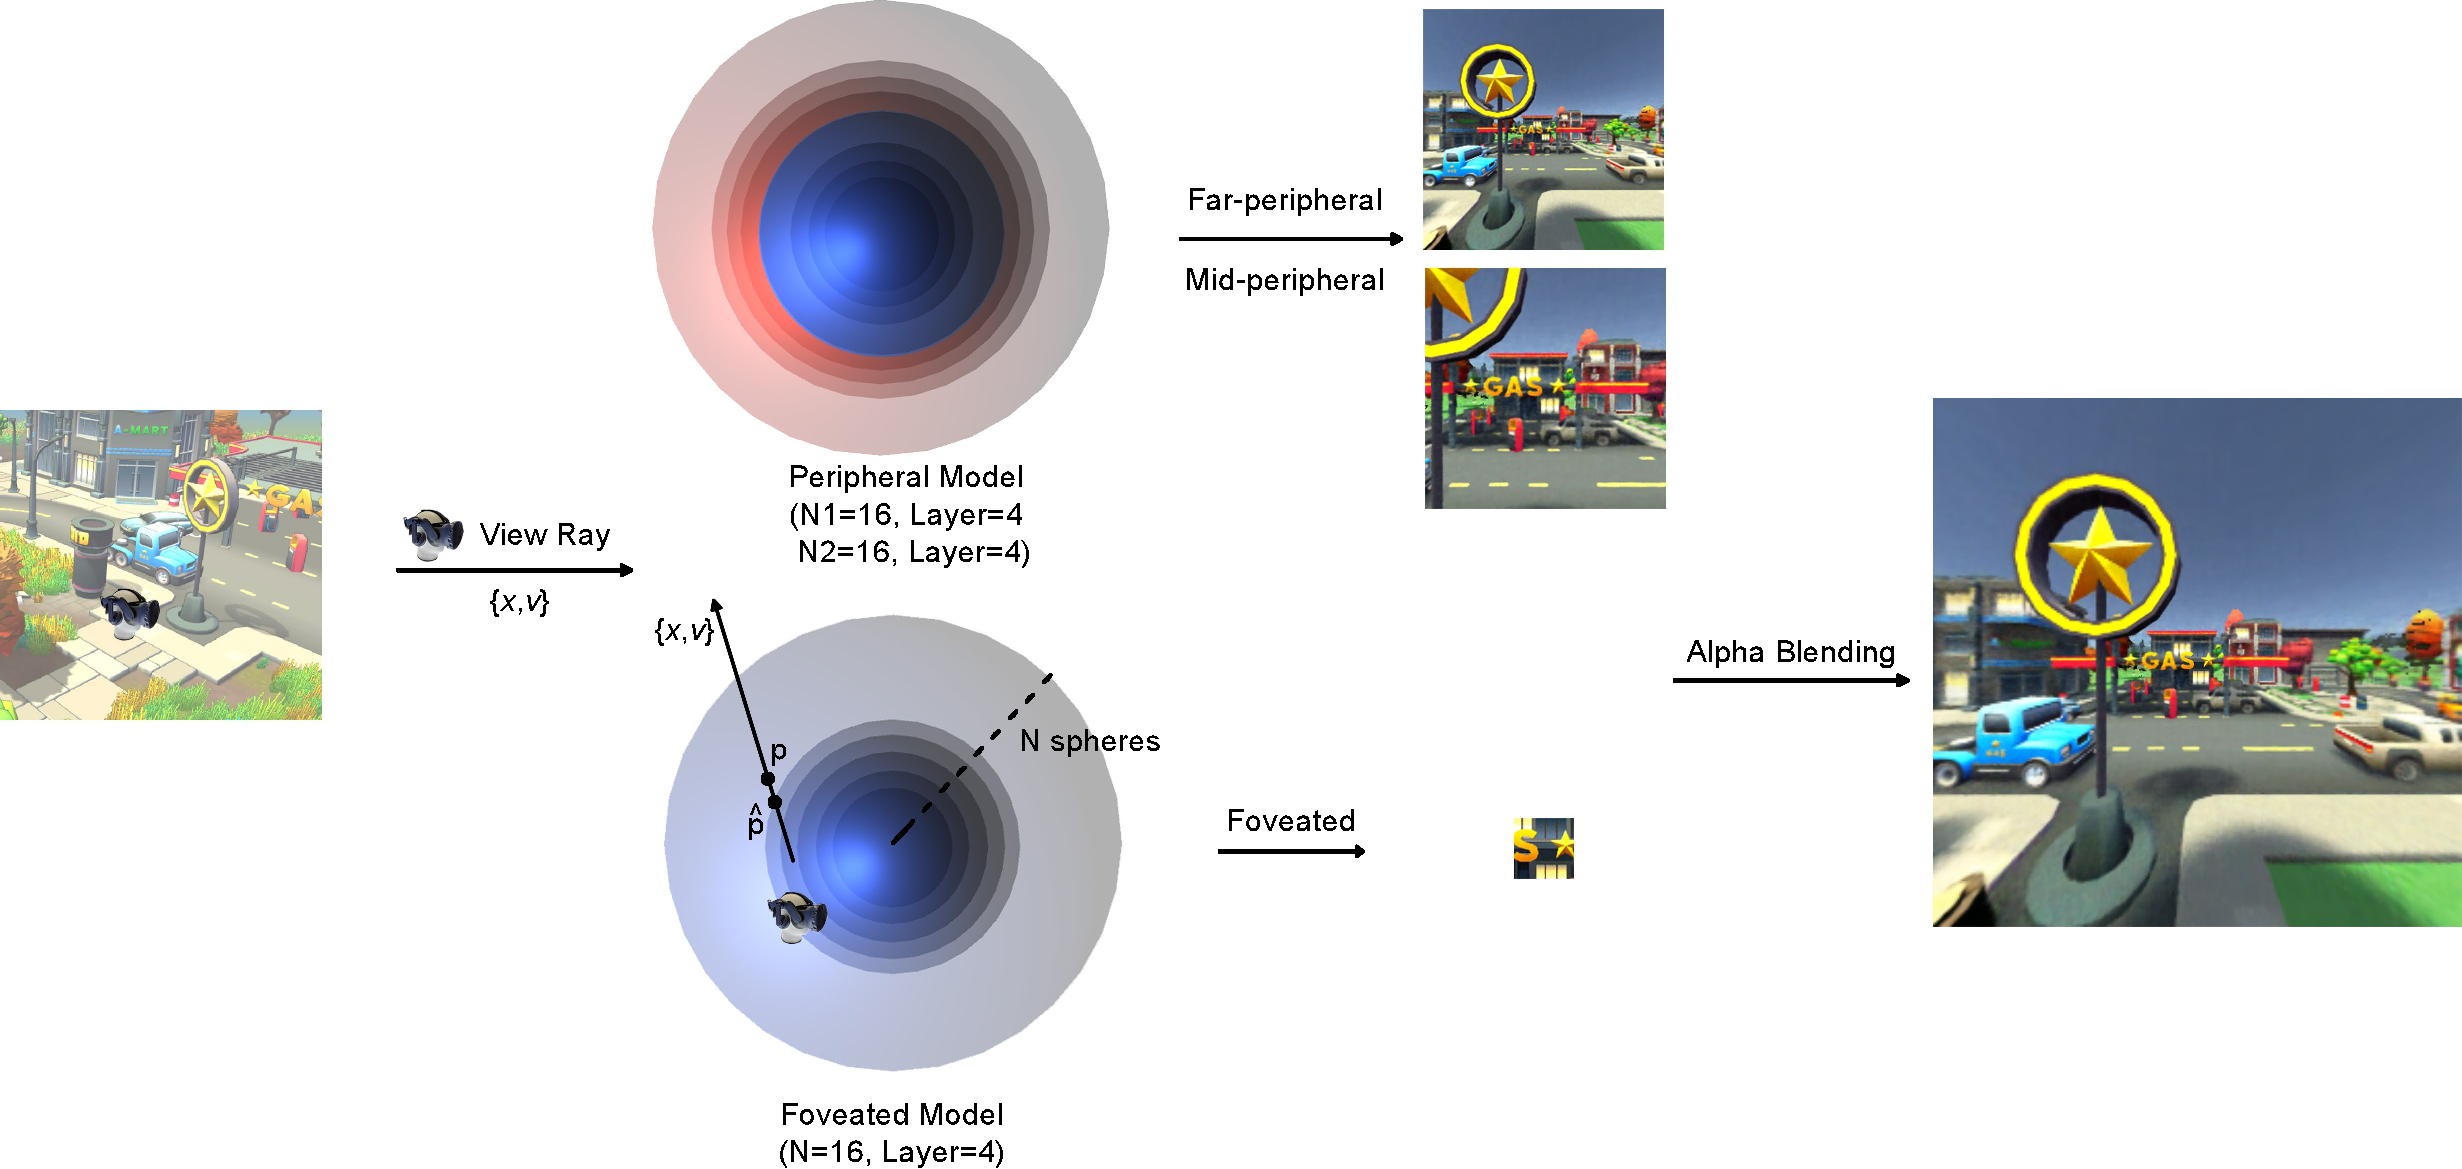
\includegraphics[width=\linewidth]{TOG/figs/pipeline.pdf}
    %\label{fig:pipeline}
    %}
    \subfloat[representation and annotation]{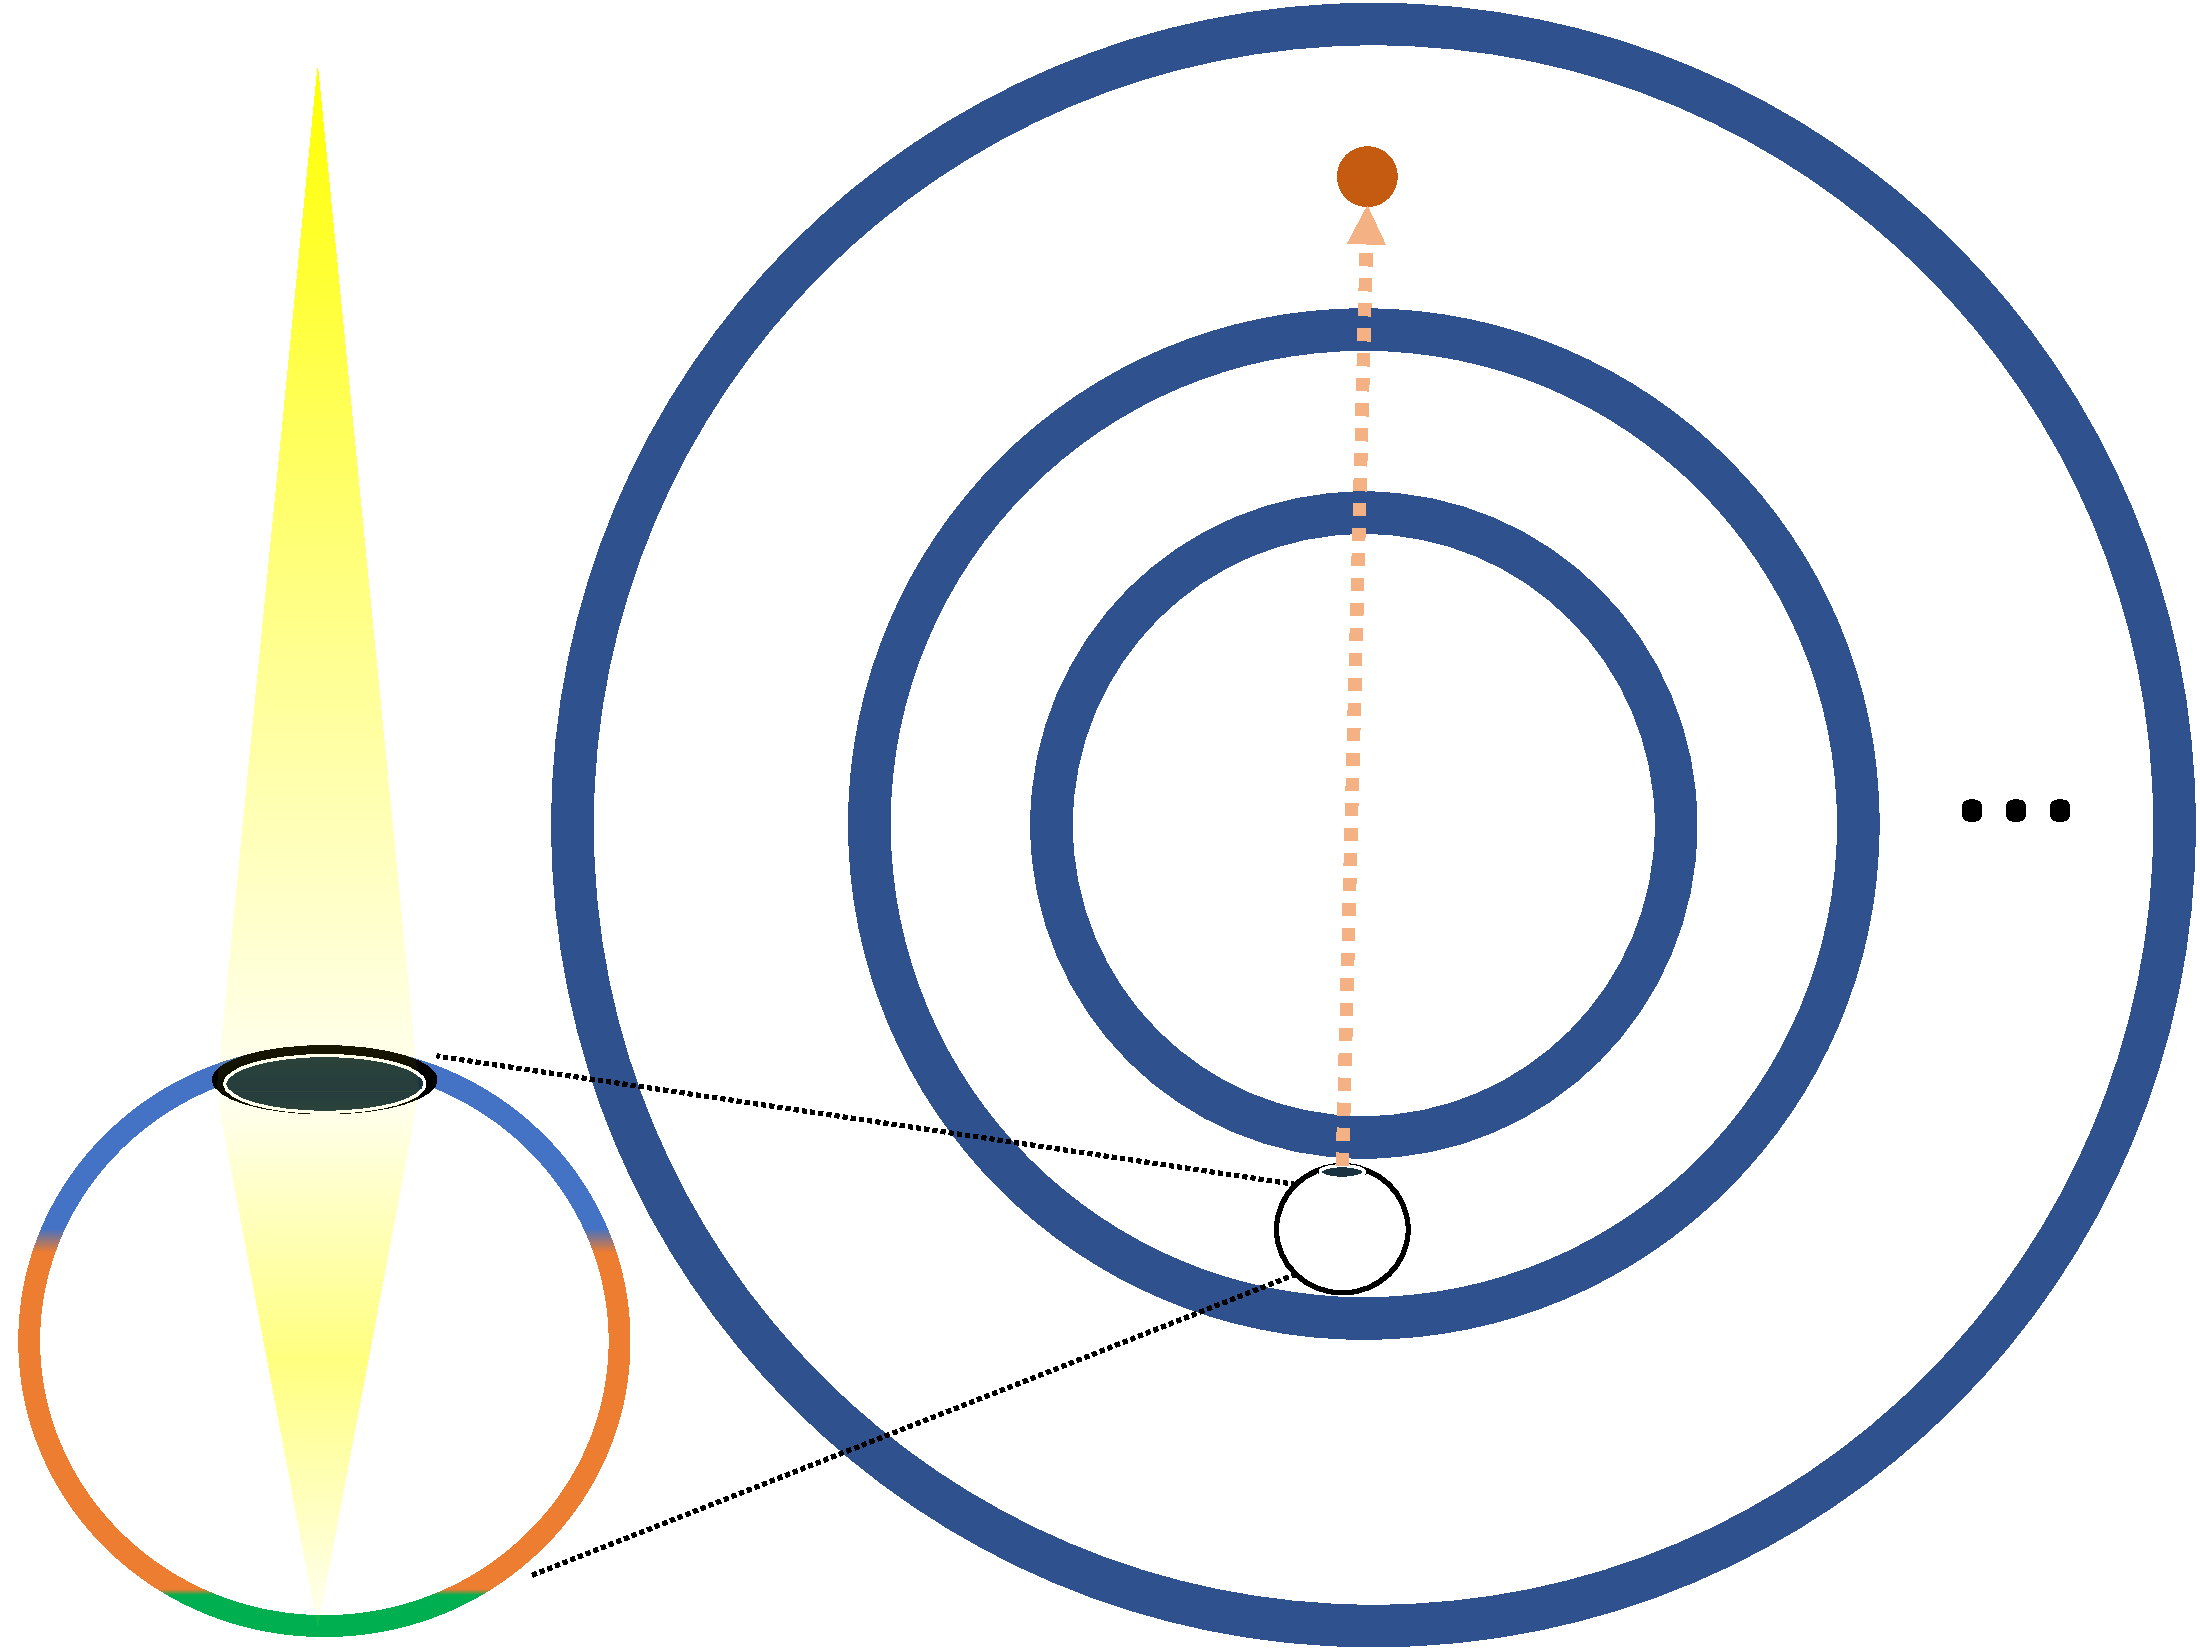
\includegraphics[width=0.8\linewidth]{TOG/figs/variables.pdf}}
    
    \subfloat[fovea]{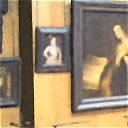
\includegraphics[width=0.3\linewidth]{TOG/figs/layer_blend/lobby_fovea.png}}\vspace{1em}
    \subfloat[mid-pheripery]{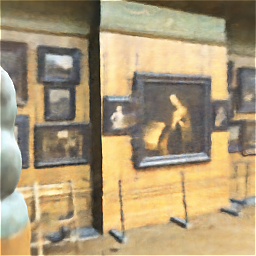
\includegraphics[width=0.3\linewidth]{TOG/figs/layer_blend/lobby_mid.png}}\vspace{1em}
    \subfloat[far-periphery]{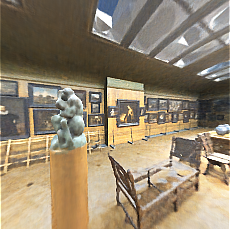
\includegraphics[width=0.3\linewidth]{TOG/figs/layer_blend/lobby_periph.png}}
    
    \subfloat[blend]{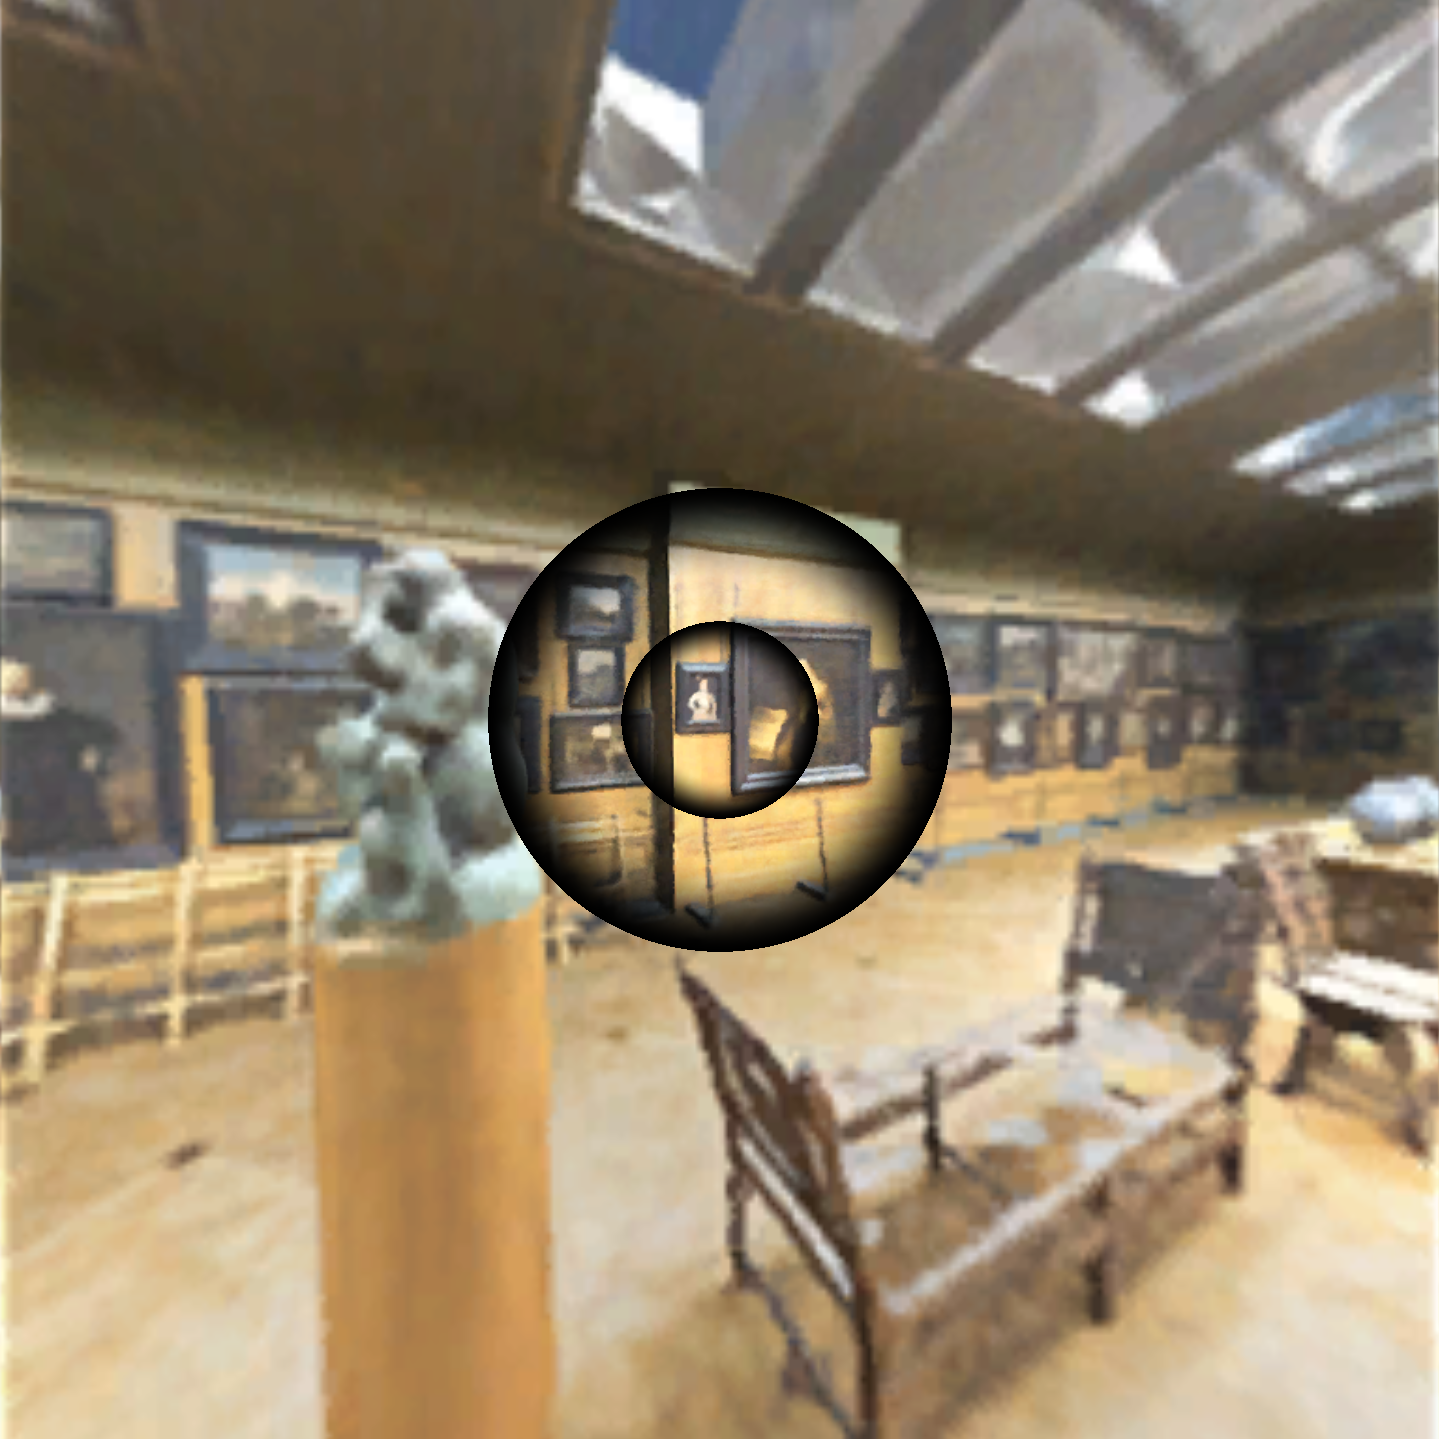
\includegraphics[width=0.9\linewidth]{TOG/figs/layer_blend/lobby_blended_with_mask.png}}
    
    %\subfloat[GazeNet]{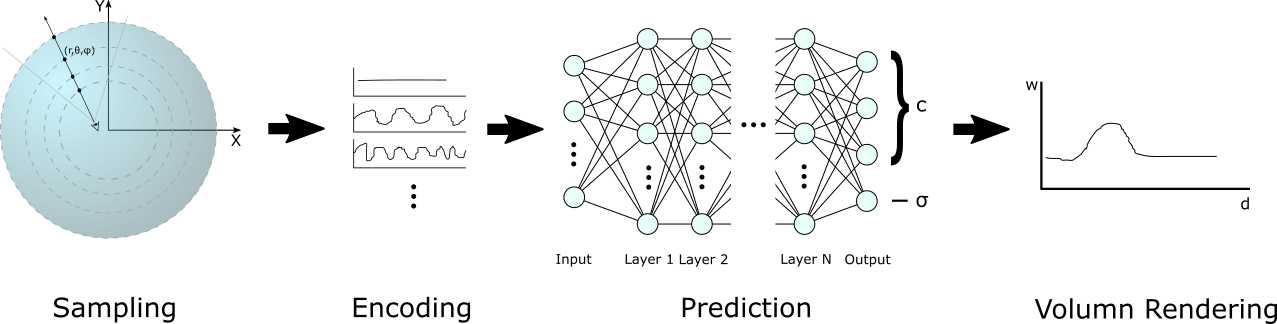
\includegraphics[width=\linewidth]{TOG/figs/spher_net_flow.png}
    %\label{fig:net}
    %}
    \Caption{System and network visualization.}
    {%
    \subref{fig:pipeline} shows breakdown of our system.
    \subref{fig:net} visualizes our neural network design.
    \warning{Label fovea, periphery FoVs in the figure}
    }
    \label{fig:system}
\end{figure}



% \subsection{First-Person Tailored Representation}
\subsection{Egocentric View Representation}
\label{sec:method:representation}
\paragraph{Multi spherical representation}
We tailor our method specifically for egocentric (first-person) view in immersive VR environments.
Unlike the object-focused ``outside-in'' view synthesis~\cite{sitzmann2019deepvoxels,mildenhall2020nerf}, rendering of immersive ``inside-out'' scenes is challenging owing to the rapid variation of scene content. As a consequence of extreme diversity among overlapping views, neural representation of large virtual scenes typically result in significant artifacts as demonstrated in \cref{fig:teaser:scene}. 
We overcome this problem by depicting the rapidly varying 360-degree virtual scenes with concentric spherical volumes. 
Inspired by \cite{Lin:DeepPanorama,Benjamin:2020:RTV}, the representation not only enables robust rendering of complex immersive environments at real-time rates, but also allows for 6DoF interaction for exploring virtual spaces, as will be discussed later.

Inspired by \cite{Broxton:immersiveLF,Lin:DeepPanorama}, we address this problem via depicting a virtual scene with concentric spherical volumes. \zh{shall we emphasize here that the root of concentric spherical volumes is the origin of the virtual scene/world?} \qisun{I intentionally didn't emphasize this part since I was wondering whether that gives people the impression of weak support of larger range translation. What do you think?}

Specifically, as shown in \Cref{fig:teaser:scene},  
%Consequently, the overlaps among views are diversified, resulting in training challenges for large virtual scenes.
%To address this problem, we depict a VR scene as concentric spherical volumes with the center as the original point, as %visualized in \Cref{fig:teaser:scene}. 
%\begin{figure}[htb]
%    \centering
%    \includegraphics[width=0.96\linewidth]{TOG/figs/spher_coord.pdf}
%%    \caption{Visualization of our multi-spherical coordinate system.}
%    \label{fig:method:coordinate}
%\end{figure}
% different position (10cm working, 50cm not working),
% different rotation
For a sphere (located at origin point) with radius $\sphereRadius$, its intersection (if exists) with a directional ray $\{\rayo,\rayd\}$ is
\begin{equation}
\pt(\sphereRadius,\rayo,\rayd) = \rayo + \left({\left((\rayo\cdot\rayd)^2-\norm{\rayo}^2+\sphereRadius^2\right)}^{\frac{1}{2}}-\rayo\cdot\rayd\right)\rayd,
    %\pt(\sphereRadius,\rayo,\rayd)=\rayo + \sphereRadius\rayd,
\end{equation}
where $\rayo$ and $\rayd$  are the ray's origin point and normalized direction respectively.
%Convert $\pt_r$ to spherical coordinate $(r, \theta, \phi)$:
%\begin{equation}
%    \begin{cases}
%        \theta = \mathrm{atan2}(x_{\pt_r}/z_{\pt_r})\\
%        \phi = \mathrm{acos}(y_{\pt_r} / r).
%    \end{cases}
%\end{equation}
%\qisun{(Jan 14) Todo for myself: I haven't done revision on this part yet. Will do so after the description becomes more understandable.}

% ZH: coordiante system? Parameterization system, parameterized representation etc.
In our first-person tailored neural representation, the scene is parameterized through the number ($\sphereNum$) and radii ($\mathbf{\sphereRadius}=\{\sphereRadius_i\},i\in [1,\sphereNum]$) of concentric spheres. Under this system, all the intersections are
\begin{equation}
\left\{\pt(\sphereRadius_i,\rayo,\rayd) \right\}\ |\ i\in[1,2,\dots,\sphereNum].
\end{equation}

Inversely, given a view point $\rayo$ observing a spatial location $\SpatialPt=\SpatialPt(\sphereRadius, \theta, \phi)$ represented in spherical coordinates, the ray connect them is with the direction $\rayd(\SpatialPt,\rayo)=\frac{\SpatialPt-\rayo}{\norm{\SpatialPt-\rayo}}$. This ray may intersect with more than one spheres. 
Among them, the closest intersection point to $\SpatialPt$ is
\begin{equation}\label{eq:closestPoint}
\begin{aligned}
    \hat{\pt}&(\rayo,\SpatialPt, \sphereNum, \mathbf{\sphereRadius}) \triangleq \\
    &\pt(\sphereRadius_k,\rayo,\rayd(\SpatialPt,\rayo))\ |\ k=\arg\min_{j\in[1,\sphereNum]}\left(\norm{\norm{\SpatialPt}-\sphereRadius_j}\right),
\end{aligned}
\end{equation}

% \begin{align}
% \pt(\sphereRadius_k,\rayo,\rayd(\SpatialPt,\rayo))\ |\ 
% k=\min (\arg\min_j(\norm{\norm{\SpatialPt}-\sphereRadius_j}), \sphereNum).
% \label{eq:intersection}
% \end{align}

The formula \Cref{eq:closestPoint} and \Cref{fig:intersection} reveal our concentric representation's spatial approximation error due to its sparsity. Specifically we compute the offset distance across all $\SpatialPt$ in a 3D static scene
\begin{equation}
\begin{aligned}
\sparseError(\sphereNum, \mathbf{\sphereRadius})  &= \iint \norm{\SpatialPt-\hat{\pt}(\rayo,\SpatialPt, \sphereNum, \mathbf{\sphereRadius})} \mathbf{d}\SpatialPt \mathbf{d}\rayo,\\
&\forall \{\rayo, \SpatialPt\} \text{ pair without occlusion in between},
\label{eq:sparseError}
\end{aligned}
\end{equation}
given it's parameters ($\sphereNum$,$\mathbf{\sphereRadius}$). Higher losses cause less precise spatial approximation, i.e., prediction error from a neural network.
Specifically, we observe
\begin{itemize}
    \item Given a fixed min/max range of $\mathbf{\sphereRadius}$, $\sphereNum$ is negatively correlated to the spatial approximation error
    \item With a fixed $\sphereNum$, the correlation between distribution of $\sphereRadius_j$ and content (i.e., distribution of $\SpatialPt$s) is positively correlated to the spatial approximation error
\end{itemize}
We determine the coordinate variables with a content-aware optimization, as further detailed in \Cref{sec:method:optimization}.

\begin{figure}
    \centering
    \subfloat[Visualization of \protect\Cref{eq:sparseError}]{\includegraphics[width = 0.47\linewidth]{example-image-a}\label{fig:intersection:visualization}}
    \subfloat[Plot]{\includegraphics[width = 0.47\linewidth]{example-image-a}}
    \caption{The relationship among $\sphereRadius$, N}
    \label{fig:intersection}
\end{figure}
%Under this definition, we obtain the nearest sphere ID of a given 3D virtual point $\pt=\pt(r, \theta, \phi)$ as:
%\begin{equation}
%    \sphereID(\pt,\sphereNum, \mathbf{\sphereRadius}) = \min (\arg\min_k(\norm{\norm{\pt}-\sphereRadius_k}), \sphereNum),
%\label{eq:sphereID}
%\end{equation}
%where $r=\norm{\pt}$  and  $\theta, \phi$ are the radius and angles of the spherical coordinate

%Consider two rays $\{\rayo_i,\rayd_i\},i=1,2$ on X axis and a point $\pt$ in 3D space. The intersections of $\pt$'s nearest sphere and the two rays are:
%\begin{equation}
%%\pt^\prime (\pt,\rayo_i,\rayd_i) = \rayo_i + \sphereRadius_{\sphereID(\pt,\sphereNum)} \rayd_i.
%\label{eq:raySphereIntersection}
%\end{equation}
%from $\rayo_1$, $\rayo_2$ to $\pt$ are $\pt'_{1,r_l}$ and $\pt'_{2,r_l}$, respectively. %$\Delta\pt'_{r_l}=\|\pt'_{2,r_l}-\pt'_{1,r_l}\|$ is small enough, then we have:
%Then, we obtain
%\begin{equation}
%\pt^\prime (\pt,\rayo_1,\rayd_1) - \pt^\prime (\pt,\rayo_2,\rayd_2) \approx 
%    \Delta\pt'_{r_l} \approx \Delta\rayo \frac{|z_\pt - r_l|}{z_\pt}
%\label{eq:deltaApprox}
%\end{equation}
%\qisun{(Jan 14, 2021) Fill in the eq. above.}

% \begin{figure}[htb]
%     \centering
%     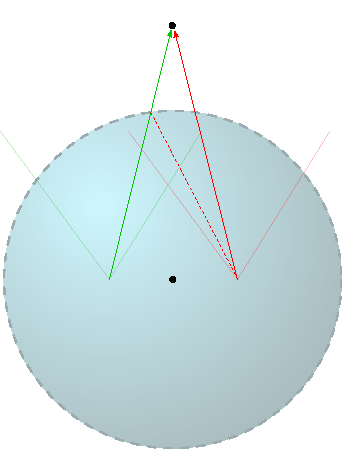
\includegraphics[width=0.96\linewidth]{TOG/figs/depth_disparity.pdf}
%     \caption{Depth disparity}
%     \label{fig:method:eccentricity}
% \end{figure}
%\qisun{(Jan 14, 2021) The figure above is not even referred in the current draft. Feel free to add them back whenever there is any real content or at least related to the textual content.}

%\begin{figure}[htb]
%    \centering
%    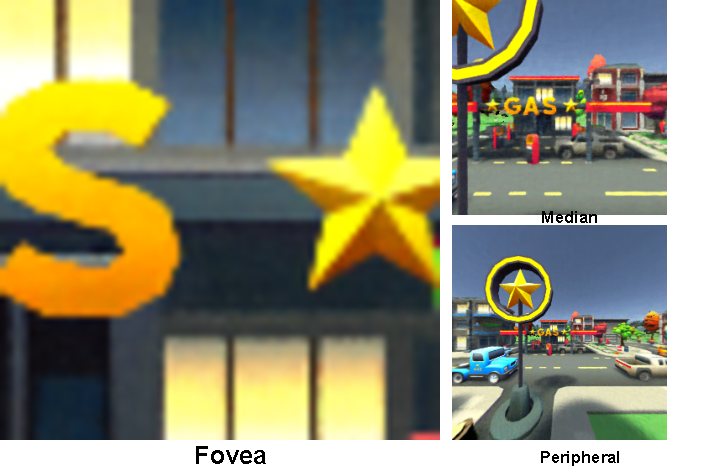
\includegraphics[width=0.96\linewidth]{TOG/figs/layers_together_zh.pdf}% try not overlapping the text on the image since we want the %reviewers to see each pixel clearly
%    \caption{Visualization of the output at three eccentricity ranges.}
%    \label{fig:method:layer}
%\end{figure}

%estimate the fovea, mid-peripheral, peripheral field of view for a novel view next, fine-tune the fovea result with local view streamed from the cloud, and lastly warp/blend the three results for VR display.
\subsection{Neural Synthesis}
Our goal is to create perceptually identical quality frames in each frame. Thus, we train networks that synthesize the foveal ($\imageFoveal(\rayo,\rayd)$, $0-10$deg), mid-peripheral ($\imageMid(\rayo,\rayd)$, $6-60$deg), and far-peripheral ($\imageFar(\rayo,\rayd)$, $60-110$deg) images in real-time.
Here, camera position $\rayo$ and gaze direction $\rayd$ are obtained from the eye-tracked HMD.

\paragraph{Input encoding}
%Since the input of our representation network is only three dimensional, we map the inputs to a higher dimensional space via high-frequency functions. \qisun{(Jan 9, 2021) What is bad if we have low-dim input? Harder to converge, higher error etc.?} \zh{(Jan 9) similar to NeRF, three components are not sufficient for achieving state-of-the-art quality, as demonstrated in Section 6.4). We introduce a positional encoding of the input coordinates that assists the MLP in
%representing high-frequency functions.}

Similar to \cite{mildenhall2020nerf}, we extend the input dimensions for higher training degree-of-freedom. This is achieved via coding the input as:
\begin{align}
\iota (p) = (\sin(2^0 p), \cos(2^0 p), ..., \sin(2^{L-1}p, \cos(2^{L-1}p))
\label{eqn:inputencode}
\end{align}
The function $\iota (\cdot)$ is applied to dimension of $\SpatialPt=(r_\SpatialPt,\theta_\SpatialPt, \phi_\SpatialPt)$.
We train the scene representation with an multilayer perception (MLP) network. 
In our experiment we choose $L=10$.\nothing{ Hence, the input dimension becomes 3 x 20 = 60 after encoding.} The MLP network is composed with $\mlpLayerNum$ fully-connected layers, each uses ReLu as activation function and $\mlpChannelNum$ channels per layer. The MLP outputs $c(\SpatialPt)\triangleq(r,g,b,d)$ for each 3D virtual voxel with our concentric parameterization in \Cref{sec:method:representation}. Here $(r,g,b)$ and $d$ represent the color and density respectively.

\paragraph{Training}
With concentric parameterization, we predicts  $c(\SpatialPt)$ for all $\SpatialPt$s along any given light ray $\{\rayo,\rayd\}$. \nothing{This follows a similar definition of \cite{mildenhall2020nerf}.} Note that besides the rays themselves, the prediction is also a function of  $\sphereNum$, $\sphereRadius_k$, and the network parameters ($\mlpLayerNum$/$\mlpChannelNum$) as evidenced in \Cref{eq:raySphereIntersection}.

Note that foveal/peripheral retinal images requires high/low pixel-wise precision but low/high FoV (number of pixels). We trained two independent neural networks that are tailored for the perceptual nature. 
%For the training uniformity and run-time efficiency, we do not distinguish different eccentricities during the training stage. Instead, the spatially variant visual acuity is represented as varying field of views in the rendering, i.e., data creation.
%Specifically, we depict the whole visual field as three retinal layers the fovea ({0-10 deg}), mid-periphery {6-60 deg}, and far periphery {60-110 deg}.
\note{
we estimate an image with size of 64 x 64, $N_{layer}=12$, $N_{channel}=64$, and $N_{sample}=16$. Regarding middle peripheral and full peripheral rendering, we estimate the two images with size of 256 x 256, $N_{layer}=8$, $N_{channel}=64$, and $N_{sample}=4$. We next upsample middle peripheral to ??? x ??? and full peripheral to 1440 x 1440 for blending.
}
Specifically, to incorporate the display hardware properties and perceptual effects, we define $\imageFoveal$/$\imageMid$/$\imageFar$ as of $64\times64$/$256\times256$/$1440\times1440$ respectively.
Thus the $\imageFoveal$ has the highest spatial resolution of \warning{xx} pixel per degree (PDD), higher than those of $\imageMid$ \warning{yy PDD} and $\imageFar$ \warning{zz}.
In each frame, three uniformized networks independently return three retinal images, as seen from the separation range in deg, gradually larger areas along eccentricity. An example is shown in \Cref{fig:system}.

\paragraph{Synthesis}
% the description of the volume density is the same as chapter 4 in NeRF paper.
After training, the nerual network is then deployed to synthesize final images via ray marching. For accelerating the performance and quality (as compared in \Cref{fig:method:bounding}), we bound the min/max of $\mathbf{\sphereRadius}$. The bounding range, together with $\sphereNum$, $\mlpLayerNum$ and $\mlpChannelNum$, are determined from a spatial-temporal optimization, as detailed in \Cref{sec:method:optimization} %The bounding, however, may introduce subtle quality drop, as shown in \Cref{fig:method:bounding}.
\begin{figure}
    \centering
    \subfloat[w bounding]{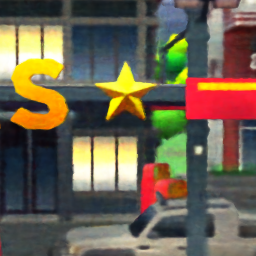
\includegraphics[width = 0.47\linewidth]{TOG/figs/depth_with_bound.png}}\hspace{1em}
    \subfloat[w/o bounding]{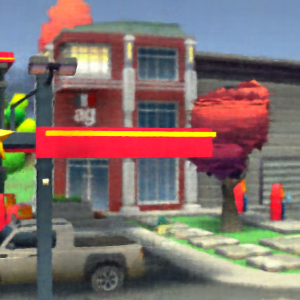
\includegraphics[width = 0.47\linewidth]{TOG/figs/depth_without_bound.png}}
    \caption{Visualization of ray marching bounding.}
    \label{fig:method:bounding}
\end{figure}
%For each pixel, we perform a ray from the camera and accumulate all the intersection's color weighted by the density accordingly between near bound and far bound. In practice, we experimented with different far bound values: 20 (meters) and 50 (meters), the difference between output is minimal. (\note{add figure for comparison}). We also experimented with the sampling number ($N_{sample}$) for accumulation between near bound and far bound to balance time cost and effects. Hence, we have an output image for the camera perspective.
 %Specifically, the network for $\imageFoveal$ generates $64\times64$ resolution (\todo{xxx} deg) with 
%However, as a gaze-contingent method, the compromised quality would be unnoticeable in periphery. Thus, we further refine the visual quality in foveal vision, as detailed in \Cref{sec:method:refine}.

\subsection{Latency-Quality Joint Optimization}
\label{sec:method:optimization}
\paragraph{3D to image space}
\Cref{eq:sparseError} depicts a generic approximation error for a given camera position and a 3D virtual space. However, typical 3D representations are not uniformly distributed points. Moreover, the network only predicts pixel colors/intensities but not depth. Thus, we further extend \Cref{eq:sparseError} to image space.
For each camera view, its projection matrix can be defined by the ray that forms with the camera's position and viewing direction $\projectionMatrix(\rayo,\rayd)$. By extending from \Cref{eq:sparseError} to the captured image space data, we obtain
\begin{align}
\imgSpaceError(\sphereNum, \mathbf{\sphereRadius}, \rayo, \rayd)  = \int \norm{\projectionMatrix(\rayo,\rayd)\cdot\SpatialPt-\projectionMatrix(\rayo,\rayd)\cdot
\pt(\sphereRadius_k,\rayo,\rayd)}\mathbf{d}\SpatialPt 
\label{eq:imageError}
\end{align}

\paragraph{Integrating with latency-introduced error}
Increasing rendering sampling naturally improves the image output quality. However, it increases the latency, causing quality drop stretched along time, and more critically, simulator sickness.
Inspired by \cite{Li:2020:TSP,albert2017latency}, we perform a spatial-temporal joint optimization to determine the spherical sampling that adapts to individual computational resources. This is achieved via a latency-precision modeling and the corresponding optimization. 

%Specifically, we model the prediction image $P$ with gaze position ($G$) at time $t$ as $P_G(t)$ and the ground truth retinal image (from a simulated local rendering) as $\hat{P}_G(t)$.
In practice, increasing the number of spheres $\sphereNum$ or number of MLP layers may affect the computational and transmissional latency but will improve the quality of individual frames (as in \Cref{eq:imageError}). Thus, we define the perceptual error as:
\begin{equation}
\begin{aligned}
&\finalError(\sphereNum, \mathbf{\sphereRadius}) = \\
&= \sum_t\int \norm{\projectionMatrix(\rayo_t,\rayd_t)\cdot\SpatialPt-\projectionMatrix(\rayo_{t-\latency},\rayd_{t-\latency})\cdot\pt(\sphereRadius_k,\rayo_{t-\latency},\rayd_{t-\latency})}\mathbf{d}\SpatialPt,
%&\int  \norm{ \imgSpaceError(\sphereNum, \mathbf{\sphereRadius}, \rayo_t, \rayd_t) - \imgSpaceError(\sphereNum, \mathbf{\sphereRadius}, \rayo_{t-l(\sphereNum, \mathbf{\sphereRadius})}, \rayd_{t-l(\sphereNum, \mathbf{\sphereRadius})})) } \mathbf{d} t
\end{aligned}
\end{equation}
where $\latency\triangleq\latency(\sphereNum, \mathbf{\sphereRadius})$ is the latency caused by alternating \warning{the representation coordinate} $\sphereNum, \mathbf{\sphereRadius}$ and network layers.

As indicated in \cite{albert2017latency}, the latency shall be below the perceptual range \warning{$L=xx$ ms}. So, we determine the optimal $\{\sphereNum, \mathbf{\sphereRadius}\}$ to balance latency and precision as
\begin{equation}
\begin{aligned}
    &\arg\min_{\sphereNum, \mathbf{\sphereRadius}} E(\sphereNum, \mathbf{\sphereRadius}), \\
    & s.t.\ {l(\sphereNum, \mathbf{\sphereRadius})} < L
\end{aligned}
\end{equation}

%$E_{q}\triangleq $
%$E_{l}$ is defined as the loss introduced by latency. 
%\begin{align}
%    \int E_{l} \mathbf{d} t
%\end{align}

\begin{figure*}
    \centering
    \subfloat[quality-only]{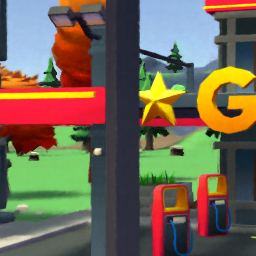
\includegraphics[width=0.3\linewidth]{TOG/figs/latency_vs_quality/quality_only.png}}\hspace{1em}
    \subfloat[latency-only]{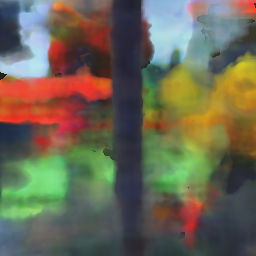
\includegraphics[width=0.3\linewidth]{TOG/figs/latency_vs_quality/latency_only.png}}\hspace{1em}
    \subfloat[ours]{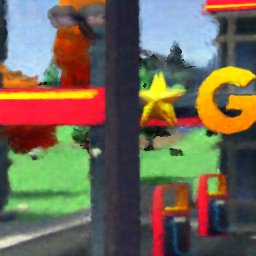
\includegraphics[width=0.3\linewidth]{TOG/figs/latency_vs_quality/our.png}}
    \caption{Latency-quality joint-optimization.}
    % talking about sample
    % (a) we need several figures with gaze movement
    \label{fig:optimization}
\end{figure*}

%\subsection{Cloud-Based System}
%\label{sec:method:system}
%Finally, we deploy our gaze-contingent synthesizer to a real-time cloud-based streaming system.

\subsection{Real-time Rendering}
% \subsection{Fovea-Peripheral Blending}
\label{sec:method:blending}
%Lastly, we apply alpha blend on the fine-tuned fovea view and middle peripheral view, as well as on the middle peripheral view and full peripheral view via function:


In real-time, the \netName predicts the two eye's projected retinal images (3 for each, 6 in total).
We then perform an image-based rendering to generate final frames for the VR head-mounted-displays.

To enhance consistency of edge area between layers, our fragment shader retrieves the three frames and applied a pixel wise bilinear interpolation at each $10\%$ connecting areas between two adjunct layers. To further preserve peripheral quality due to its low PDD, we enhanced the contrast following the mechanism of \cite{Patney:2016:TFR}, the details are visualized in \Cref{fig:method:blending}.

\begin{figure}
    \centering
    \subfloat[blending]{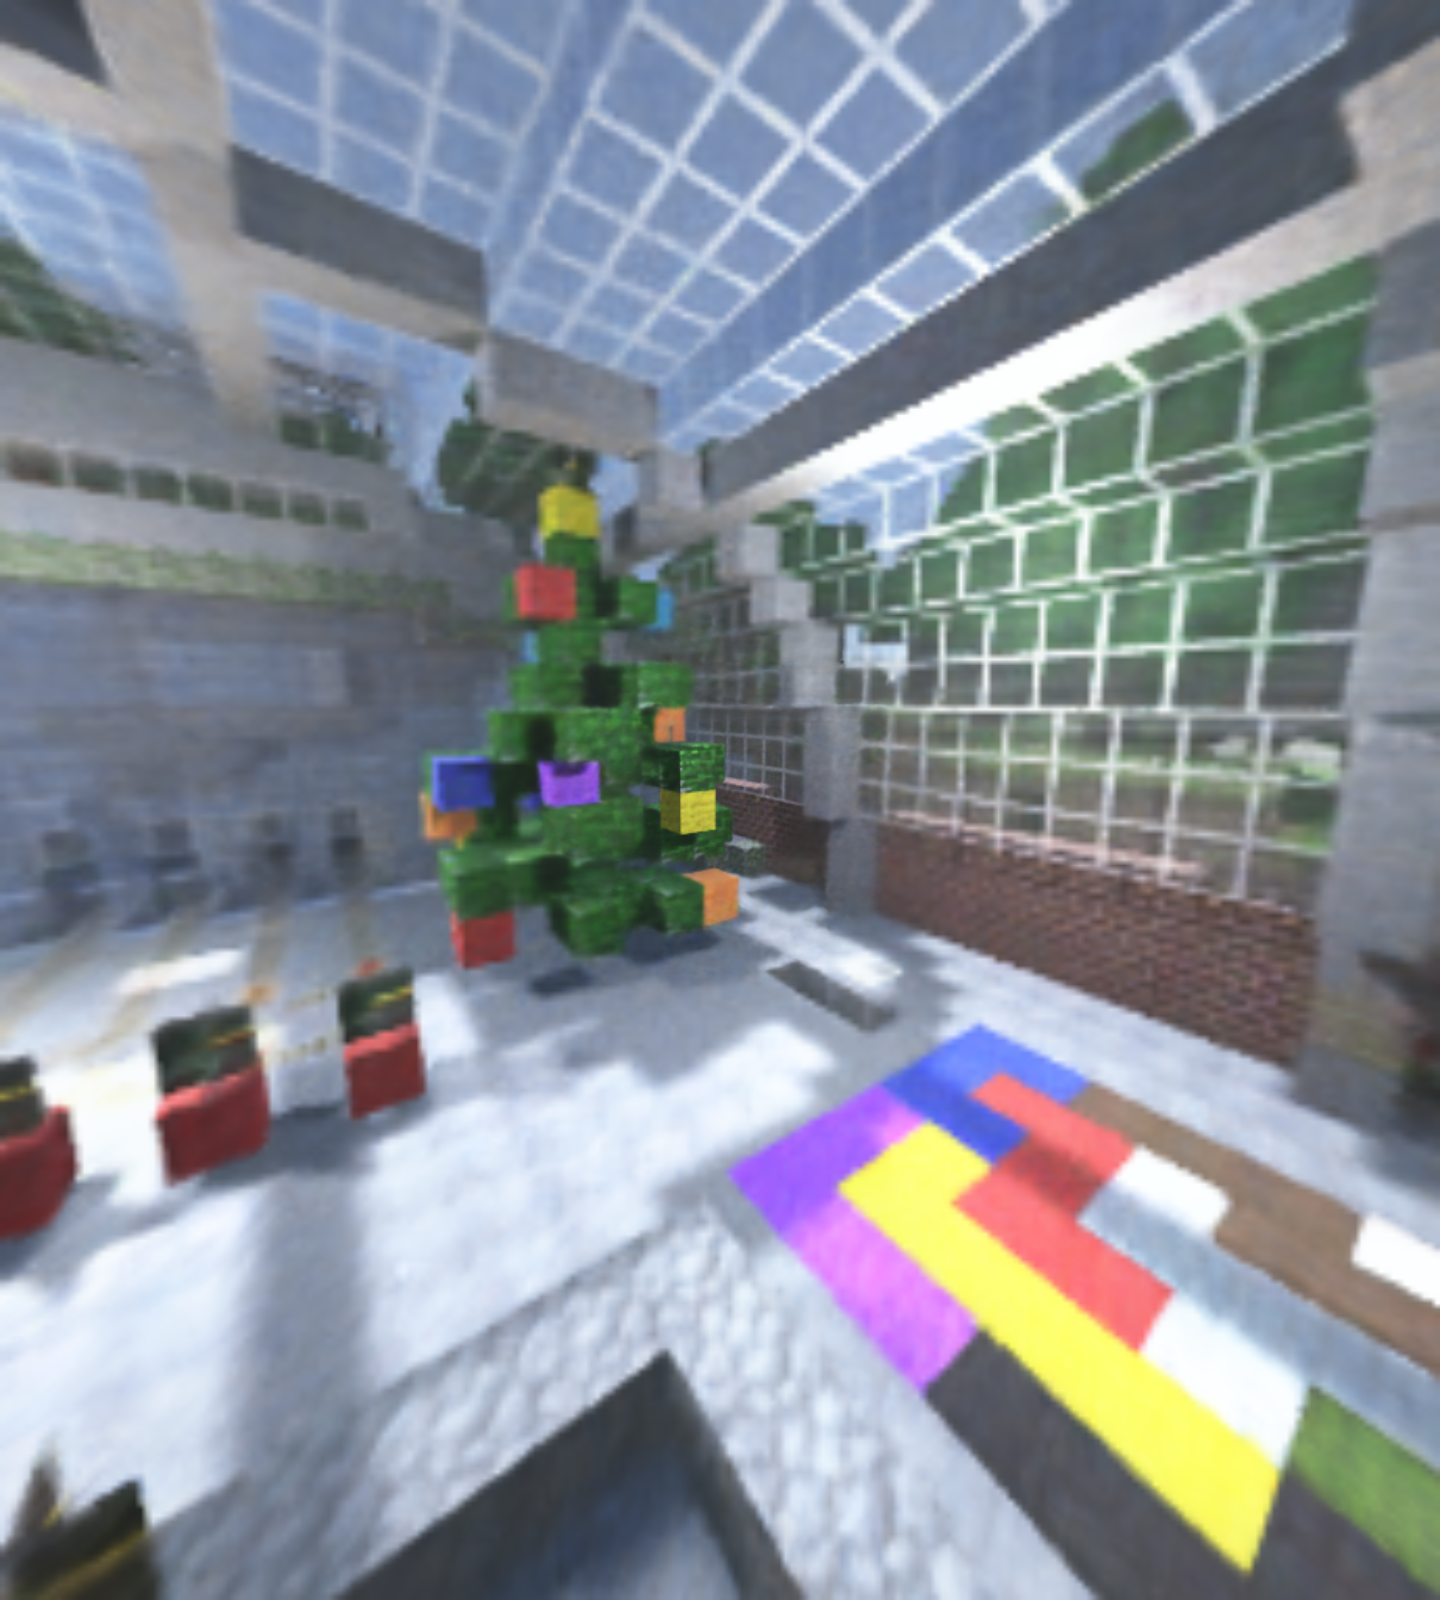
\includegraphics[width = 0.8\linewidth]{TOG/figs/system/blended.png}}

    \subfloat[Contrast enhancement]{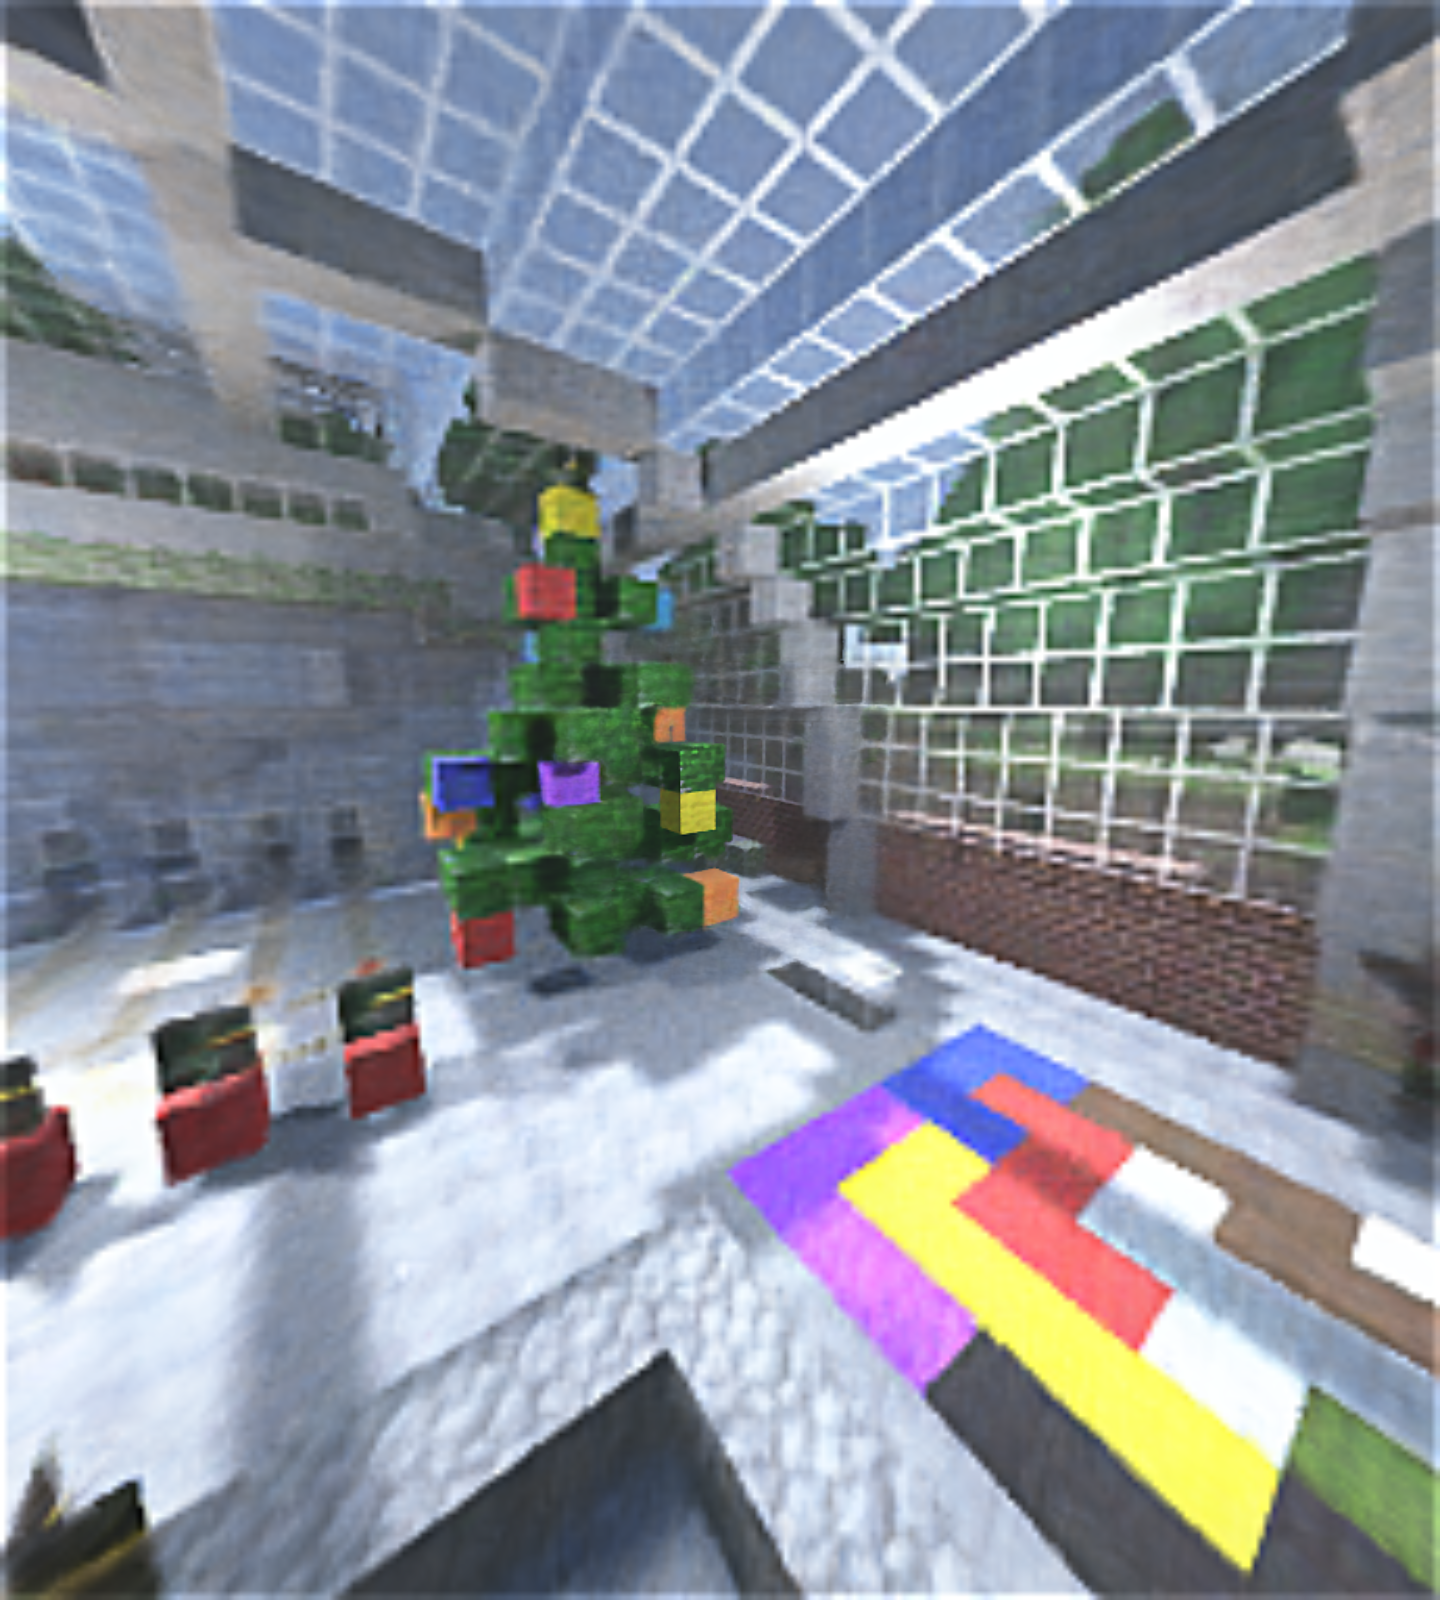
\includegraphics[width = 0.8\linewidth]{TOG/figs/system/blended_enhanced.png}}
    \caption{Our multi-layer real-time rendering system.\zh{Or three-image pipeline}}
    \label{fig:method:blending}
\end{figure}

\nothing{
\subsection{Refinement for Fovea Layer}
\label{sec:method:refine}
Due to the depth bounding and prediction errors, it is particularly challenging to preserve pixel-wise quality without compromising real-time performance. However, the human foveal vision is remarkably sensitive to subtle details across all frequency ranges. To 
To maximize the quality of foveated image, we utilize the limited but consistent network bandwidth by retrieving a local peripheral image from the cloud. The retrieval was realized by cloud-based rendering using users' upstreamed head and gaze parameters.
Due to the inevitable dual-way transmission, it is impossible to instantly obtain the image without latency. Displaying outdated frames have been studied as a major cause of simulator sickness.
}%nothing
\note{describe when to retrieve new full peripheral image.} We leverage local guidance views to fine tune the output foveated image. Local guidance view is decided according to current camera view. We chose the nearest 4 views (or 8 views) as reference views and estimate the color as well as volume density for all reference views. Every time we receive a new peripheral image from the cloud, we calculate the delta between the ground truth and our result for reference views for preparation. Then we warp the delta into target camera view, calculate the average and apply to the fovea result for each frame.

\section{Implementation}
\paragraph{Data generation}

\paragraph{Parameters}
\zh{different network impl for peripheral @Nianchen}

\paragraph{Environment}
We implement our neural network with pytorch and the rendering system in Unity.
The system was experimented with a Windows machine with \warning{Intel i9-7900X CPU @ 3.30 GHz}, 64GB RAM and one NVIDIA GTX 3080 graphics card.